
免责声明:敬请大家仔细对比本模版与官方word转pdf后的差别,自行确定是否采用。
取消正文tex这一行注释即可对比:\verb|%\renewcommand{\input}[1]|\\
\verb|{\vspace{\baselineskip}}|。
个人认为,2025年系统仍然上传PDF,只要人眼无法分辨与官方区别,就可以。

\subsection{编译方法}
\begin{enumerate}
	\item 编译:XeLaTex->bibtex->XeLaTeX->XeLaTeX
	\item 排错:多看编译错误,多查询错误解决方法;编译警告,只要不影响PDF,就不用管。本模版多人使用,可以认为不存在编译错误。
	\item 自定义格式:多阅读一下nsfc.sty,可以解决你绝大部分问题。超过nsfc.sty范围的,建议不要想办法定制,事倍功半。
\end{enumerate}


\subsection{编辑方法}
%%%%%%%%
%\newpage
\vspace{-5pt}

\begin{figure}[h!]
	\centering %图片居中
	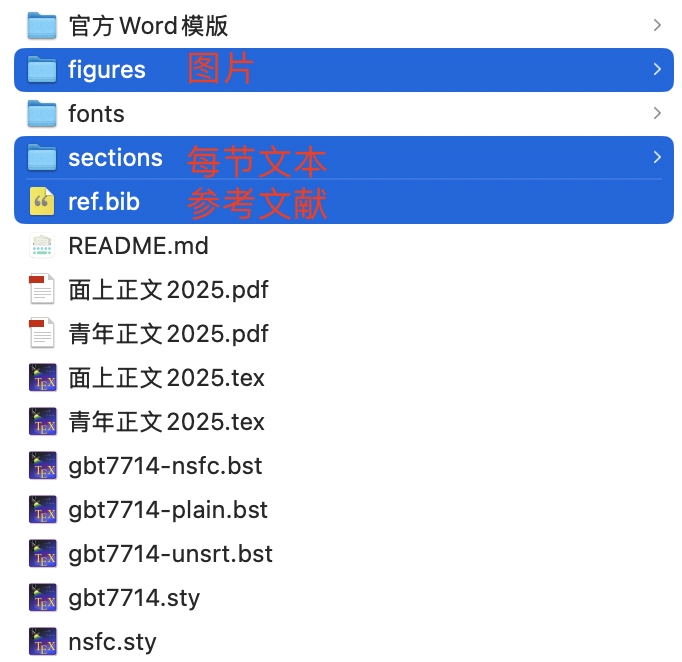
\includegraphics[width=6cm]{figures/xiugai.png}
	\captionsetup{justification=centering} %图题居中
	\caption{项目文件夹结构。}
\end{figure}
只需要修改上图中蓝色选中区域文件即可。其他剩余文件,可以直接采用模版替换,编译就是最新版。

\subsubsection{章节}\label{subsubsec:t}
\verb|\label{subsubsect:t}|
引用章节\verb|\ref{subsubsec:t}|,生成为:\ref{subsubsec:t}。这个样式可能不是你想要的,那种情况下,就手敲吧!申请书不像论文,这种情况应该没几个。

\subsubsection{字体}
中文\textbf{粗体};\textbf{bold} font;
中文\textit{斜体};\textit{italic} font;

全文改宋体,可以修改nsfc.sty的MS部分字体。

可选的就是\verb|\zhkai,\enkai,\zhsong,\ensong|。

\subsubsection{文献}
% 普通引用\cite{test};上标引用\citess{test};多篇文章\citess{test,test2,test3}。

% 有注音的英文:\cite{test}。

% 参考期刊\cite{test};
% 参考图书\cite{test2};
% 参考会议\cite{test5};
% 参考链接\cite{test4};
% 参考文件\cite{test6}。

% 对于中文参考文献,bib条目中需要有language = {zh},参见\cite{test2}。
\subsubsection{列表}
无序列表\footnote{值得注意的是,不需要一定要用列表环境,用加粗、换行、缩进同样能达到效果。
	因为咱们的初衷,还是LaTeX在排版文献和公式上有优势,发挥这一个优势就行了,其他部分不需要强行套用。文本本身还是最重要、需要大家投入精力的部分。}的例子:
\begin{itemize}[left= 50pt]
	\item[-] 第一条,第一条的内容可能很长长长长长长长长长长长长长长长长长长长长;
	\item[-] 第二条。
\end{itemize}

有序列表的例子:
\begin{enumerate}[left= 50pt]
	\item 第一条,第一条的内容可能很长长长长长长长长长长长长长长长长长长长长;
	\item 第二条。
\end{enumerate}

两个带圈文字的实现方法:
\textcircled{\raisebox{-0.8pt}{1}}
\textcircled{\textbf{\small 1}}

注意,由于列表的缩进,不同使用者可能偏向并不一样。本模版用的enumitem包,阅读他的文档进行个性化,其文档在:https://www.ctan.org/pkg/enumitem


\subsubsection{公式}

公式如下:
\begin{equation}
	E=mc^2
\end{equation}
公式的上下间距参见nsfc.sty中公式上下间距部分。

\subsubsection{图}
图片的例子:
\begin{figure}[h!]
\centering %图片居中
\includegraphics[width=2cm]{figures/IMG.JPG}
\captionsetup{justification=centering} %图题居中
\caption{这是图题。}
\end{figure}

图题和表头若想取消加粗,去掉nsfc.sty中caption部分的\verb|\bfseries|即可。


\subsubsection{表}
在表格内的第一行设置\verb|\zhkai\ensong\selectfont|,来选择字体。

其中\verb|\zhkai\zhsong\enkai\ensong|可以根据需要选择。
\begin{table}[htbp]
	\zhkai\ensong\selectfont%设置表格字体
	\centering  % 显示位置为中间
	\caption{表格}  % 表格标题
	\label{table1}  % 用于索引表格的标签
	%字母的个数对应列数,|代表分割线
	% l代表左对齐,c代表居中,r代表右对齐
	\begin{tabular}{|c|c|c|c|}  
		\hline  % 表格的横线
		& & & \\[-6pt]  %可以避免文字偏上来调整文字与上边界的距离
		第一列&第二列&第三列&第四列 \\  % 表格中的内容,用&分开,\\表示下一行
		\hline
		& & & \\[-6pt]  %可以避免文字偏上 
		0.1&0.2&0.3&0.4 \\
		\hline
	\end{tabular}
\end{table}

\subsection{某页最后一段行距可能很窄?}
如果没有这个问题,就不用管这个事情。

行间距变化一般是在“多行蓝色模版”部分前后。因为蓝色模版文字在section里写的,latex把蓝色部分当作一个整体,可能硬要挤到这一页,而不是换新一页,导致会挤前一页的行间距,导致前一页行距异常。
针对这种情况,模版已经使用
\begin{lstlisting}[language=tex, basicstyle=\ttfamily\small, keywordstyle=\color{blue}, commentstyle=\color{gray}]
	%自动段落的行间距微调
	\usepackage{setspace}
	\setstretch{1.6} % 22 bp / 14 pt = 1.571
\end{lstlisting}
降低了这种情况发生的可能。
如果还有,就只好添加\verb|\newpage|把它newpage到后一页上,就行了。也可以考虑分段缓解,需要写的时候注意页面的分段和字数。

\begin{REF}
\subsection*{参考文献}
\vspace{-50pt}
\bibliographystyle{gbt7714-nsfc}
\bibliography{ref}%参考文献
\end{REF}

\newpage%自己判断是否需要
